% Hlavicka pro protokoly z fyzikalniho praktika.
% Verze pro: LaTeX
% Verze hlavicky: 22. 2. 2007
% Autor: Ustav fyziky kondenzovanych latek
% Ke stazeni: www.physics.muni.cz/ufkl/Vyuka/
% Licence: volne k pouziti, nejlepe k vcasnemu odevzdani protokolu z Vaseho mereni.

\documentclass[a4paper,11pt]{article}

% Kodovani (cestiny) v dokumentu: utf-8
%\usepackage[cp1250]{inputenc}	% Omezena stredoevropska kodova stranka, pouze MSW.
\usepackage[utf8]{inputenc}	% Doporucujeme pouzivat UTF-8 (unicode).
\usepackage[T1]{fontenc}
\usepackage{lmodern}

%%% Nemente:
\usepackage[margin=2cm]{geometry}
\newtoks\jmenopraktika \newtoks\jmeno \newtoks\datum
\newtoks\obor \newtoks\skupina \newtoks\rocnik \newtoks\semestr
\newtoks\cisloulohy \newtoks\jmenoulohy
\newtoks\tlak \newtoks\teplota \newtoks\vlhkost
\usepackage{amsmath}
\usepackage{mathtools}
\usepackage{graphicx}
\usepackage{multirow}

\usepackage{pgfplotstable} 
\usepackage{booktabs}

\graphicspath{ {./images/} }
%%% Nemente - konec.


%%%%%%%%%%% Doplnte pozadovane polozky:

\jmenopraktika={Fyzikální praktikum 3}  % nahradte jmenem vaseho predmetu
\jmeno={Artem Gorodilov}            % nahradte jmenem mericiho
\datum={20. ~května  2024}        % nahradte datem mereni ulohy
\obor={Astrofyzika}                     % nahradte zkratkou vami studovaneho oboru
\skupina={Po 14:00}            % nahradte dobou vyuky vasi seminarni skupiny
\rocnik={II}                  % nahradte rocnikem, ve kterem studujete
\semestr={II}                 % nahradte semestrem, ve kterem studujete

\cisloulohy={D}               % nahradte cislem merene ulohy
\jmenoulohy={Franck-Hertzův experiment } % nahradte jmenem merene ulohy

\tlak={979}                   % nahradte tlakem pri mereni (v hPa)
\teplota={21.4}               % nahradte teplotou pri mereni (ve stupnich Celsia)
\vlhkost={46}               % nahradte vlhkosti vzduchu pri mereni (v %)

%%%%%%%%%%% Konec pozadovanych polozek.


%%%%%%%%%%% Uzitecne balicky:
\usepackage[czech]{babel}
\usepackage{graphicx}
\usepackage{amsmath}
\usepackage{xspace}
\usepackage{url}
\usepackage{indentfirst}
\usepackage{listings}
\usepackage{subcaption}
\usepackage{caption}
\usepackage{tabularx}
\usepackage[labelformat=parens,labelsep=quad,skip=3pt]{caption}

%%%%%% Zamezeni parchantu:
\widowpenalty 10000 \clubpenalty 10000 \displaywidowpenalty 10000
%%%%%% Parametry pro moznost vsazeni vetsiho poctu obrazku na stranku
\setcounter{topnumber}{3}	  % max. pocet floatu nahore (specifikace t)
\setcounter{bottomnumber}{3}	  % max. pocet floatu dole (specifikace b)
\setcounter{totalnumber}{6}	  % max. pocet floatu na strance celkem
\renewcommand\topfraction{0.9}	  % max podil stranky pro floaty nahore
\renewcommand\bottomfraction{0.9} % max podil stranky pro floaty dole
\renewcommand\textfraction{0.1}	  % min podil stranky, ktery musi obsahovat text
\intextsep=8mm \textfloatsep=8mm  %\intextsep pro ulozeni [h] floatu a \textfloatsep pro [b] or [t]

% Tecky za cisly sekci:
\renewcommand{\thesection}{\arabic{section}.}
\renewcommand{\thesubsection}{\thesection\arabic{subsection}.}
% Jednopismenna mezera mezi cislem a nazvem kapitoly:
\makeatletter \def\@seccntformat#1{\csname the#1\endcsname\hspace{1ex}} \makeatother

\begin{document}

\thispagestyle{empty}

{
\begin{center}
\sf 
{\Large Ústav fyzikální elektroniky PřF MU} \\
\bigskip
{\huge \bfseries FYZIKÁLNÍ PRAKTIKUM} \\
\bigskip
{\Large \the\jmenopraktika}
\end{center}

\bigskip

\sf
\noindent
\setlength{\arrayrulewidth}{1pt}
\begin{tabular*}{\textwidth}{@{\extracolsep{\fill}} l l}
\large {\bfseries Zpracoval:}  \the\jmeno & \large  {\bfseries Naměřeno:} \the\datum\\[2mm]
\large  {\bfseries Obor:} \the\obor  \hspace{40mm}  {\bfseries Skupina:} \the\skupina %
%{\bfseries Ročník:} \the\rocnik \hspace{5mm} {\bfseries Semestr:} \the\semestr  
&\large {\bfseries Testováno:}\\
\\
\hline
\end{tabular*}
}

\bigskip

{
\sf
\noindent \begin{tabular}{p{3cm} p{0.6\textwidth}}
\Large  Úloha č. {\bfseries \the\cisloulohy:} \par
\smallskip
% $T=\the\teplota$~$^\circ$C \par
% $p=\the\tlak$~hPa \par
% $\varphi=\the\vlhkost$~\%
&\Large \bfseries \the\jmenoulohy  \\[2mm]
\end{tabular}
}

\vskip10pt
    \begin{minipage}[t]{0.5\textwidth} 
        \section{Zadání}    
            \begin{enumerate}
                \item Sledovat vliv nastavení experimentu na chování proudu procházejícího trubicí.
                \item Změřit závislost anodového proudu na urychlujícím napětí a určit energii nejnižší excitační
                hladiny atomů vzácného plynu v trubici.
                \item Naměřit spektrum vyzařované z trubice Franck-Hertzova experimentu a určit, jaký plyn
                v trubici září.
            \end{enumerate}
        \section{Teorie}
            \subsection{Franck-Hertzův experiment}
                \par Franck-Hertzův experiment je jedním z prvních experimentů, který dokázal kvantovou povahu atomů. Při průchodu elektronů přes plynnou trubici dochází k excitaci atomů plynu. Elektrony jsou urychlovány elektrickým polem a při dostatečně vysoké energii mohou předat energii atomům plynu. Při předání energie dochází k excitaci atomů a následně k jejich deexcitaci. Při deexcitaci dochází k emisi fotonů, které jsou detekovány. 
                \par Při průchodu elektronů plynnou trubicí dochází k vytvoření proudu, který je závislý na urychlujícím napětí. Při určitém napětí dojde k náhlému poklesu proudu, což je způsobeno tím, že elektrony předají energii atomům plynu a dojde k excitaci. Tento jev se nazývá Franck-Hertzův jev.
            \subsection{Energie excitační hladiny}
                \par Energie excitační i-hladiny atomů plynu je dána vztahem:
    \end{minipage}
    \hspace{10pt}
    \begin{minipage}[t]{0.5\textwidth} 
                \begin{equation}
                    E_{ex, i} = e \frac{U_i}{i}
                \end{equation}
                kde $e$ je elementární náboj a $U_i$ je urychlující napětí v daném maximu proudu $i$ viz. obrázek (\ref{fig:rtut}).

                \vspace{10pt}   
                \par \centering
                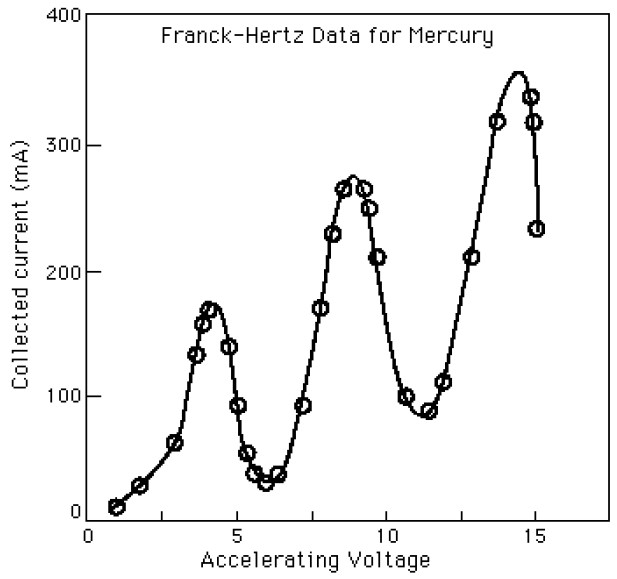
\includegraphics[scale=0.5]{rtut}
                \captionsetup{justification=centering, font=footnotesize}
                \captionof{figure}{Závislost kolektorového proudu na urychlujícím napětí pro rtut'.}
                \label{fig:rtut}
                \vspace{10pt}
                \raggedright 

            \subsection{Experementální uspořádání}
                \par Experimentální uspořádání Franck-Hertzova experimentu je zobrazeno na obrázku (\ref{fig:scheme}). Elektrony jsou emitovány z rozžhavené katody, stabilizovány kalibračním napětím $U_1$, poté urychleny anodovým napětím $U_2$ a nakonec zpomaleny brzdným napětím $U_3$. Při průchodu elektronů plynovou trubicí jsou atomy plynu excitovány a poté deexcitovány. Během deexcitace jsou emitovány a zaznamenávány fotony. 
                
    \end{minipage}
\newpage
    \begin{minipage}[t]{0.5\textwidth} 
                \vspace{0pt}   
                \par \centering
                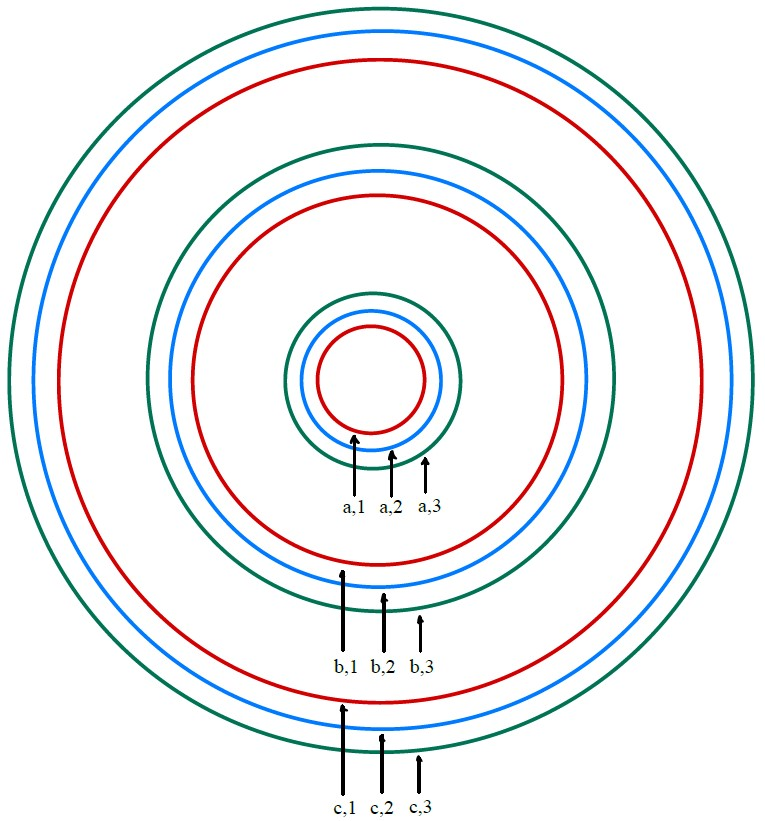
\includegraphics[scale=0.4]{scheme}
                \captionsetup{justification=centering, font=footnotesize}
                \captionof{figure}{Experimentální uspořádání Franck-Hertzova experimentu.}
                \label{fig:scheme}
                \vspace{10pt}
                \raggedright

        \section{Měření}   
            \subsection{Nalezení optimálních parametrů experimentu}
                Pro nalezení optimálních hodnot $U_1$ a $U_3$ jsme zkoumali závislost $I$ = $f(U_2)$. Za tímto účelem jsme zafixovali $U_1$ a změnili hodnotu $U_3$, poté jsme totéž zopakovali v opačném pořadí. Současně jsme sledovali změnu proudu $I$. Naším cílem bylo najít takové hodnoty $U_1$ a $U_3$, při kterých se ručička ampérmetru v daném rozsahu hodnot (od 0 A do 10,5 A) třikrát vychýlila, čímž jsme získali tři vrcholy na V-A charakteristice.

                \par Tímto způsobem jsme zjistili následující optimální hodnoty $U_1$ a $U_3$: 
                \begin{center}
                    $U_1$ = 2.5 V, $U_3$ = 8.14 V.
                \end{center}

            \subsection{Měření závislosti $I$ = $f(U_2)$}
                Po nastavení požadovaných optimálních parametrů systému jsme změřili a vykreslili závislost $I$ = $f(U_2)$ a fitovali polynomem oblasti proudových špiček. Výsledky jsou znázorněny na grafu (\ref{fig:peaks}) a v tabulce (1).

                \vspace{10pt}   
                \par \centering
                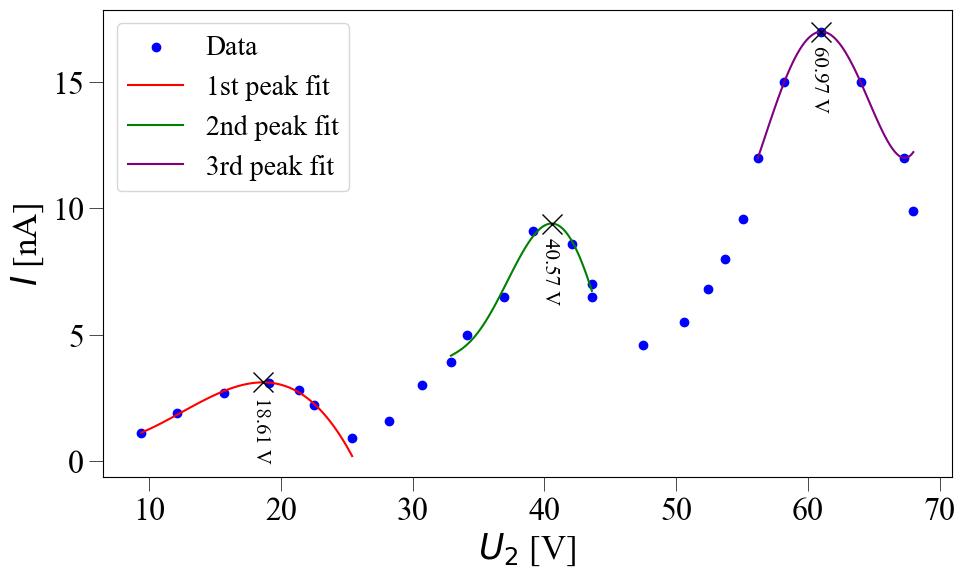
\includegraphics[scale=0.33]{peaks}
                \captionsetup{justification=centering, font=footnotesize}
                \captionof{figure}{Závislost kolektorového proudu na urychlujícím napětí.}
                \label{fig:peaks}
                \vspace{10pt}
                \raggedright 
    \end{minipage}
    \hspace{10pt}
    \begin{minipage}[t]{0.5\textwidth} 
                Získali jsme následující hodnoty datových maxim: 
                \begin{center}
                    \begin{tabular}{c|c|c}
                        \hline
                        $U_2$ [V] & $I$ [nA] & E [eV] \\
                        \hline
                        18.61(8) & 3.11(1) & 18.61(8) \\
                        40.57(5) & 8.40(3) & 20.29(3) \\
                        61.97(6) & 17.00(4) & 20.32(2) \\
                        \hline
                    \end{tabular}
                \end{center}

                Podle vzorce (1) jsme tedy zjistili hodnotu energie excitační hladiny atomů plynu:
                \begin{center}
                    $E_{ex, min}$ = 19.7(6) eV
                \end{center}

            \subsection{Určení prvků plynu}
                K určení prvků s nejbližší hodnotou nejnižší excitované energie atomu plynu, kterou jsme získali, jsme použili databázi $NIST ASD$ \cite{nist_ads}.
                \par Zjistili jsme, že prvky s nejbližší hodnotou $E_{ex, min}$ jsou:
                \begin{center}
                    $E_{He I}$ = 19.82 eV ~a~ $E_{Ne I}$ = 16.62 eV.
                \end{center}

                Abychom nakonec určili prvek plynu, změřili jsme spektrum měřeného plynu a vytvořili spektra prvků He I a Ne I pomocí databáze $NIST LIBS$ \cite{nist_libs}. Poté jsme spektra vynesli do jednoho grafu, abychom vizuálně analyzovali jejich podobnost. Výsledky jsou uvedeny na obrázku (\ref{fig:spec}). 

                \par K výpočtu veličin a jejich nejistot byla použita knihovna Uncertinties pro Python \cite{uncertainties}. Chyby byly rozšířeny o Studentův koeficient (2-Tail Confidence Level) s ohledem na stupně volnosti pro každou hodnotu, pro interval spolehlivosti 68.27\%.

        \section{Závěr}
                \par Při hledání optimálních parametrů experimentu jsme stanovili následující funkce napětí: Při zvyšování $U_1$ proud $I$ zvyšuje, což je způsobeno tím, že větší množství elektronů je fokusováno tak aby prošlo trubicí. Při zvyšování $U_3$ proud $I$ zvyšuje, což je způsobeno tím, že větší množství elektronů je zpomaleno a může předat energii atomům plynu. Optimalní hodnoty $U_1$ a $U_3$ byly 2.5 V a 8.14 V.
                \par Z naměřených hodnot jsme určili energii nejnižší excitační hladiny atomů plynu, která byla rovna $E_{ex, min}$ = 19.7(6) eV. 
                \par Na základě výsledků jsme určili, že prvkem plynu je, pravděpodobně, Ne I. Pro potvrzení jsme změřili spektrum měřeného plynu a porovnali jsme ho s databází $NIST LIBS$. Většina spektrálních čar měřeného plynu odpovídala spektru prvku Ne I, což potvrzuje naše předchozí tvrzení.
                \par Rozdíl mezi $E_{ex, min}$ a $E_{Ne I}$ byl 3.1(6) eV což může být způsobeno chybou měření kvůli oscilacím proudu, které mohou být způsobeny nečistotami v trubici nebo nepřesnost v nastavení optimálních parametrů napětí.
    \end{minipage}
\newpage
                \vspace{10pt}   
                \par \centering
                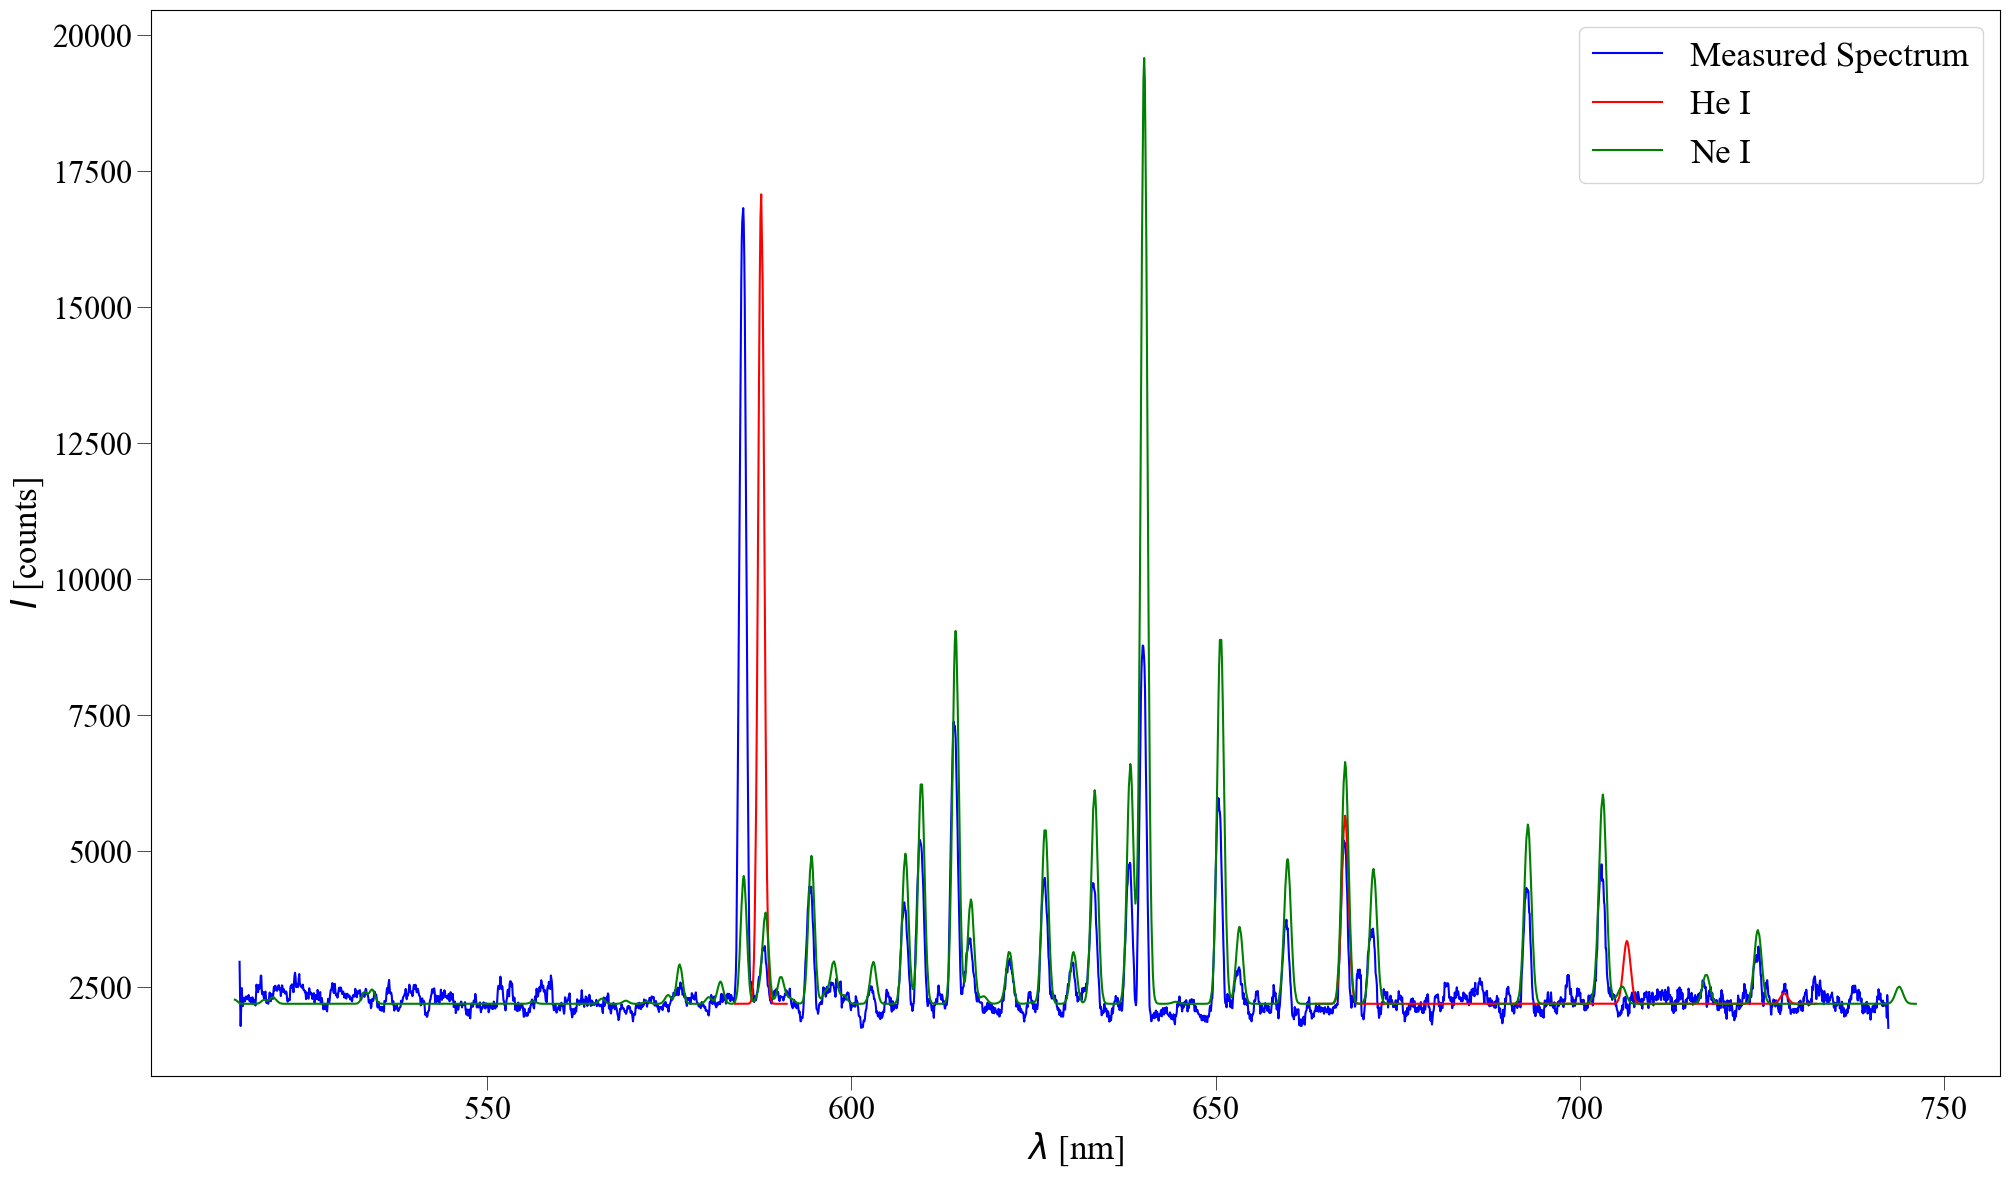
\includegraphics[scale=0.33]{spec}
                \captionsetup{justification=centering, font=footnotesize}
                \captionof{figure}{Spektra měřeného plynu a prvků He I a Ne I.}
                \label{fig:spec}
                \vspace{10pt}
                \raggedright 

                \renewcommand{\refname}{Odkazy}
                \begin{thebibliography}{9}
                    \bibitem{nist_ads}
                        NIST ASD, Dostupné online: \url{https://physics.nist.gov/PhysRefData/ASD/lines_form.html}
                    \bibitem{nist_libs}
                        NIST LIBS, Dostupné online: \url{https://physics.nist.gov/PhysRefData/ASD/LIBS/libs-form.html}
                    \bibitem{uncertainties}
                        Uncertainties, Dostupné online: \url{https://pypi.org/project/uncertainties}
                \end{thebibliography} 

    \begin{center}
        \section{Appendix}
            \subsection{Tabulka naměřených hodnot pro spektrální čáry železa}
                \pgfplotstabletypeset[
                col sep=comma, % Defines the separator, comma for CSV
                string type, % Treats columns as strings (not math mode)
                every head row/.style={before row=\toprule,after row=\midrule},
                every last row/.style={after row=\bottomrule},
                columns/U/.style={column name=$U_2$ [V]},
                columns/I/.style={column name=$I$ [nA]},
                ]{data/VA_proc.csv}
    \end{center}
\end{document}